\documentclass[a4paper, 14pt]{extarticle}

\usepackage[T2A]{fontenc}
\usepackage[utf8]{inputenc}
\usepackage[english, russian]{babel}
\usepackage{amsmath}
\usepackage{subcaption}
\usepackage{graphicx}
\usepackage{float}
\usepackage{hyperref}

\usepackage[left=3cm, right=1.5cm, top=2cm, bottom=2cm]{geometry}
\usepackage{setspace}
\onehalfspacing 

\usepackage{indentfirst}
\setlength{\parindent}{1.25cm} 
\setlength{\emergencystretch}{3em}
\usepackage[expansion=false,protrusion=false,nopatch=footnote]{microtype}

\usepackage{tocloft}
\addto\captionsrussian{\renewcommand{\contentsname}{СОДЕРЖАНИЕ}}
\renewcommand{\cfttoctitlefont}{\hfill\normalfont}
\renewcommand{\cftaftertoctitle}{\hfill\vspace{\baselineskip}}
\renewcommand{\cftsecdotsep}{\cftdotsep}

\begin{document}

\begin{titlepage}
    \begin{center}
        Министерство науки и высшего образования Российской Федерации\\
        Федеральное государственное автономное образовательное учреждение высшего образования\\
        «Санкт-Петербургский политехнический университет Петра Великого»\\
        
        \textbf{Физико-механический институт}\\
        \textbf{Высшая школа прикладной математики и вычислительной физики}
    \end{center}

    \vfill
    
    \begin{center}
        \textbf{Отчёт по лабораторной работе \textnumero~ 1\\[0.5cm]}
        \textbf{Гистограммы и плотности распределений\\}
        по дисциплине <<Математическая статистика>>
    \end{center}

    \vfill

    \hfill
    \begin{minipage}{0.45\textwidth}
        \textbf{Выполнил студент гр. 5030102/30202:}\\
        Шильдт Д.С.\\[0.5cm]
        \textbf{Преподаватель:}\\ 
        Баженов А.Н.
    \end{minipage}

    \vfill

    \begin{center}
        Санкт-Петербург\\2026
    \end{center}
\end{titlepage}

\setcounter{page}{2}

\tableofcontents
\newpage

\section{Постановка задачи}

Сгенерировать выборки объемом $n = 10, 100, 1000$ для каждого из пяти следующих распределений:
\begin{enumerate}
    \item Нормальное $N(x;0,1)$
    \item Коши $C(x;0,1)$
    \item Лапласа $L(x;0,\frac{1}{\sqrt{2}})$
    \item Пуассона $P(k;10)$
    \item Равномерное $U(x;-\sqrt{3}, \sqrt{3})$
\end{enumerate}
Для каждой сгенерированной выборки нужно построить на одном графике гистограмму и теоретическую кривую плотности распределения и сделать вывод о том, как объем выборки влияет на возможность распознавания характера распределения.

\section{Теоретическая часть}

В данной лабораторной работе исследуются пять видов распределений: четыре непрерывных и одно дискретное. Ниже приведены их функции плотности и основные теоретические сведения \cite{babakhina, maksimov}.
\subsection{Теоретические сведения о распределениях}

\textbf{1. Нормальное распределение} $N(x; \mu, \sigma)$
Плотность вероятности имеет вид:
\begin{equation*}
    f(x) = \frac{1}{\sigma\sqrt{2\pi}} \exp\left(-\frac{(x-\mu)^2}{2\sigma^2}\right)
\end{equation*}
В задании используется стандартное нормальное распределение с параметрами $\mu = 0$ и $\sigma = 1$.

\textbf{2. Распределение Коши} $C(x; x_0, \gamma)$
Плотность вероятности задается формулой:
\begin{equation*}
    f(x) = \frac{1}{\pi\gamma \left[1 + \left(\frac{x-x_0}{\gamma}\right)^2\right]}
\end{equation*}
Параметры для генерации: параметр сдвига $x_0 = 0$, параметр масштаба $\gamma = 1$.

\textbf{3. Распределение Лапласа} $L(x; \beta, \alpha)$
Плотность вероятности:
\begin{equation*}
    f(x) = \frac{\alpha}{2} e^{-\alpha|x-\beta|}
\end{equation*}
Для работы используются параметр сдвига $\beta = 0$ и масштабный параметр $\frac{1}{\alpha} = \frac{1}{\sqrt{2}}$ (соответственно, $\alpha = \sqrt{2}$).

\textbf{4. Распределение Пуассона} $P(k; \lambda)$
Является дискретным распределением. Вероятность того, что случайная величина примет значение $k$ ($k = 0, 1, 2, \dots$), равна:
\begin{equation*}
    P(X = k) = \frac{\lambda^k}{k!}e^{-\lambda}
\end{equation*}
В задании используется математическое ожидание $\lambda = 10$.

\textbf{5. Равномерное распределение} $U(x; a, b)$
Плотность вероятности задается кусочно:
\begin{equation*}
    f(x) =
    \begin{cases}
        \frac{1}{b-a}, & x \in [a, b] \\
        0, & x \notin [a, b]
    \end{cases}
\end{equation*}
Параметры для выборки: $a = -\sqrt{3}$, $b = \sqrt{3}$.

Основные числовые характеристики используемых распределений сведены в таблицу \ref{tab:distributions}. Параметры непрерывных распределений подобраны таким образом, чтобы их математическое ожидание равнялось $0$, а дисперсия равнялась $1$.

\begin{table}[h]
    \centering
    \caption{Числовые характеристики исследуемых распределений}
    \label{tab:distributions}
    \resizebox{\textwidth}{!}{%
    \begin{tabular}{|l|c|c|c|}
        \hline
        \textbf{Распределение} & \textbf{Параметры} & \textbf{Математическое ожидание $M(X)$} & \textbf{Дисперсия $D(X)$} \\ \hline
        Нормальное & $\mu=0, \sigma=1$ & 0 & 1 \\ \hline
        Коши & $x_0=0, \gamma=1$ & Не существует & Не существует \\ \hline
        Лапласа & $\beta=0, \alpha=\sqrt{2}$ & 0 & 1 \\ \hline
        Пуассона & $\lambda=10$ & 10 & 10 \\ \hline
        Равномерное & $a=-\sqrt{3}, b=\sqrt{3}$ & 0 & 1 \\ \hline
    \end{tabular}%
    }
\end{table}

\subsection{Теория построения гистограмм}
    
Для построения гистограммы диапазон значений случайной величины $[a, b]$, где $a = x_{min}$, $b = x_{max}$, разбивается на $k$ интервалов. Для каждого разряда вычисляется количество попаданий элементов выборки $m_l$. Затем вычисляется относительная частота попаданий $p_l$ \cite{babakhina}:
\begin{equation*}
    p_l = \frac{m_l}{n}, \quad l = 1, \dots, k
\end{equation*}
где $n$ — общий объем выборки \cite{babakhina}.

Ключевым моментом при построении является выбор оптимального числа интервалов $k$ (бинов). Если взять слишком мало разрядов, график получится неинформативным из-за потери информации. Если разрядов слишком много, данных в каждом интервале может оказаться недостаточно, что приведет к визуальному шуму на графике \cite{babakhina}. Для определения оптимального количества интервалов часто применяется полуэмпирическая формула Старджесса \cite{maksimov}:
\begin{equation*}
    k \approx 1 + 3.3 \lg n
\end{equation*}

\section{Реализация}

\subsection{Язык программирования и среда}
    \begin{itemize}
        \item \textbf{Используемый язык:} Python 3.14.2
        \item \textbf{Используемая среда разработки:} Visual Studio Code
    \end{itemize}

\subsection{Используемые библиотеки}
    \begin{itemize}
        \item \textbf{numpy} --- использовалась для работы с массивами данных и математическими функциями.
        \item \textbf{scipy} --- использовалась для генерации выборок из теоретических распределений и вычисления функций плотности/вероятности.
        \item \textbf{matplotlib} --- использовалась для визуализации данных и построения гистограмм.
        \item \textbf{pathlib} --- использовалась для автоматического создания каталогов и сохранения итоговых графиков.
    \end{itemize}

\subsection{Суть реализованных методов}
Программная реализация сводится к генерации выборок объемом $n \in \{10, 100, 1000\}$ для каждого из пяти распределений и их визуальному сравнению с теоретическими законами. Для генерации данных использовались распределения из модуля \texttt{scipy.stats} (\texttt{norm}, \texttt{cauchy}, \texttt{laplace}, \texttt{poisson}, \texttt{uniform}). Для получения выборок применялся метод \texttt{.rvs()}.
Для получения точек теоретической кривой у непрерывных распределений вызывался метод \texttt{.pdf()}. Исключением стало распределение Пуассона: поскольку оно является дискретным, теоретические вероятности вычислялись с помощью метода \texttt{.pmf()}.

\textbf{1. Вспомогательные функции визуализации:}
\begin{itemize}
    \item \texttt{vizData(ax, data, x, y, n, bins='auto', is\_discrete=False)} — функция для визуализации данных. Она строит эмпирическую гистограмму выборки. С помощью флага \texttt{is\_discrete} реализовано ветвление: для непрерывных величин теоретическая плотность отрисовывается в виде плавной линии, а для дискретных — в виде маркеров-точек.
    \item \texttt{finalizeFigure(fig, dist\_name)} — функция для финальной компоновки и экспорта графиков.
\end{itemize}

\textbf{2. Функции анализа конкретных распределений:}
\begin{itemize}
    \item \texttt{normDistribution(sizes)} --- отвечает за анализ нормального распределения $N(0,1)$. Генерирует выборки и вычисляет теоретическую плотность на отрезке $[-4,4]$.
    \item \texttt{cauchyDistribution(sizes)} --- реализует анализ распределения Коши $C(0,1)$. Поскольку теоретические моменты у данного распределения не существуют, генерация сопровождается экстремальными выбросами. Поэтому в функции предусмотрена фильтрация: для визуализации берутся только значения из интервала $[-10,10]$. Это сохраняет читаемость гистограммы.
    \item \texttt{laplaceDistribution(sizes)} --- функция для распределения Лапласа $L(0,\frac{1}{\sqrt{2}})$. Работает на отрезке $[-10,10]$. Для корректной генерации в методы библиотеки \texttt{scipy} передаются параметр сдвига \texttt{loc=0} и параметр масштаба \texttt{scale=1/np.sqrt(2)}.
    \item \texttt{poissonDistribution(sizes)} --- функция для дискретного распределения Пуассона $P(k;10)$.
    \item \texttt{uniformDistribution(sizes)} --- отвечает за равномерное распределение $U(-\sqrt{3},\sqrt{3})$. В методы генерации передаются параметр левой границы \texttt{loc=-np.sqrt(3)} и параметр ширины интервала \texttt{scale=2*np.sqrt(3)}.
\end{itemize}

\section{Результаты}
Для каждого из пяти исследуемых законов распределения построены графики, совмещающие гистограмму относительных частот (по выборкам объемом $n \in \{10, 100, 1000\}$) и соответствующую теоретическую кривую плотности вероятности.

На рис.~\ref{fig:norm} приведены результаты для нормального распределения, на рис.~\ref{fig:cauchy} --- для распределения Коши, на рис.~\ref{fig:laplace} --- для распределения Лапласа, на рис.~\ref{fig:poisson} --- для распределения Пуассона, на рис.~\ref{fig:uniform} --- для равномерного распределения.

\begin{figure}[H]
    \centering
    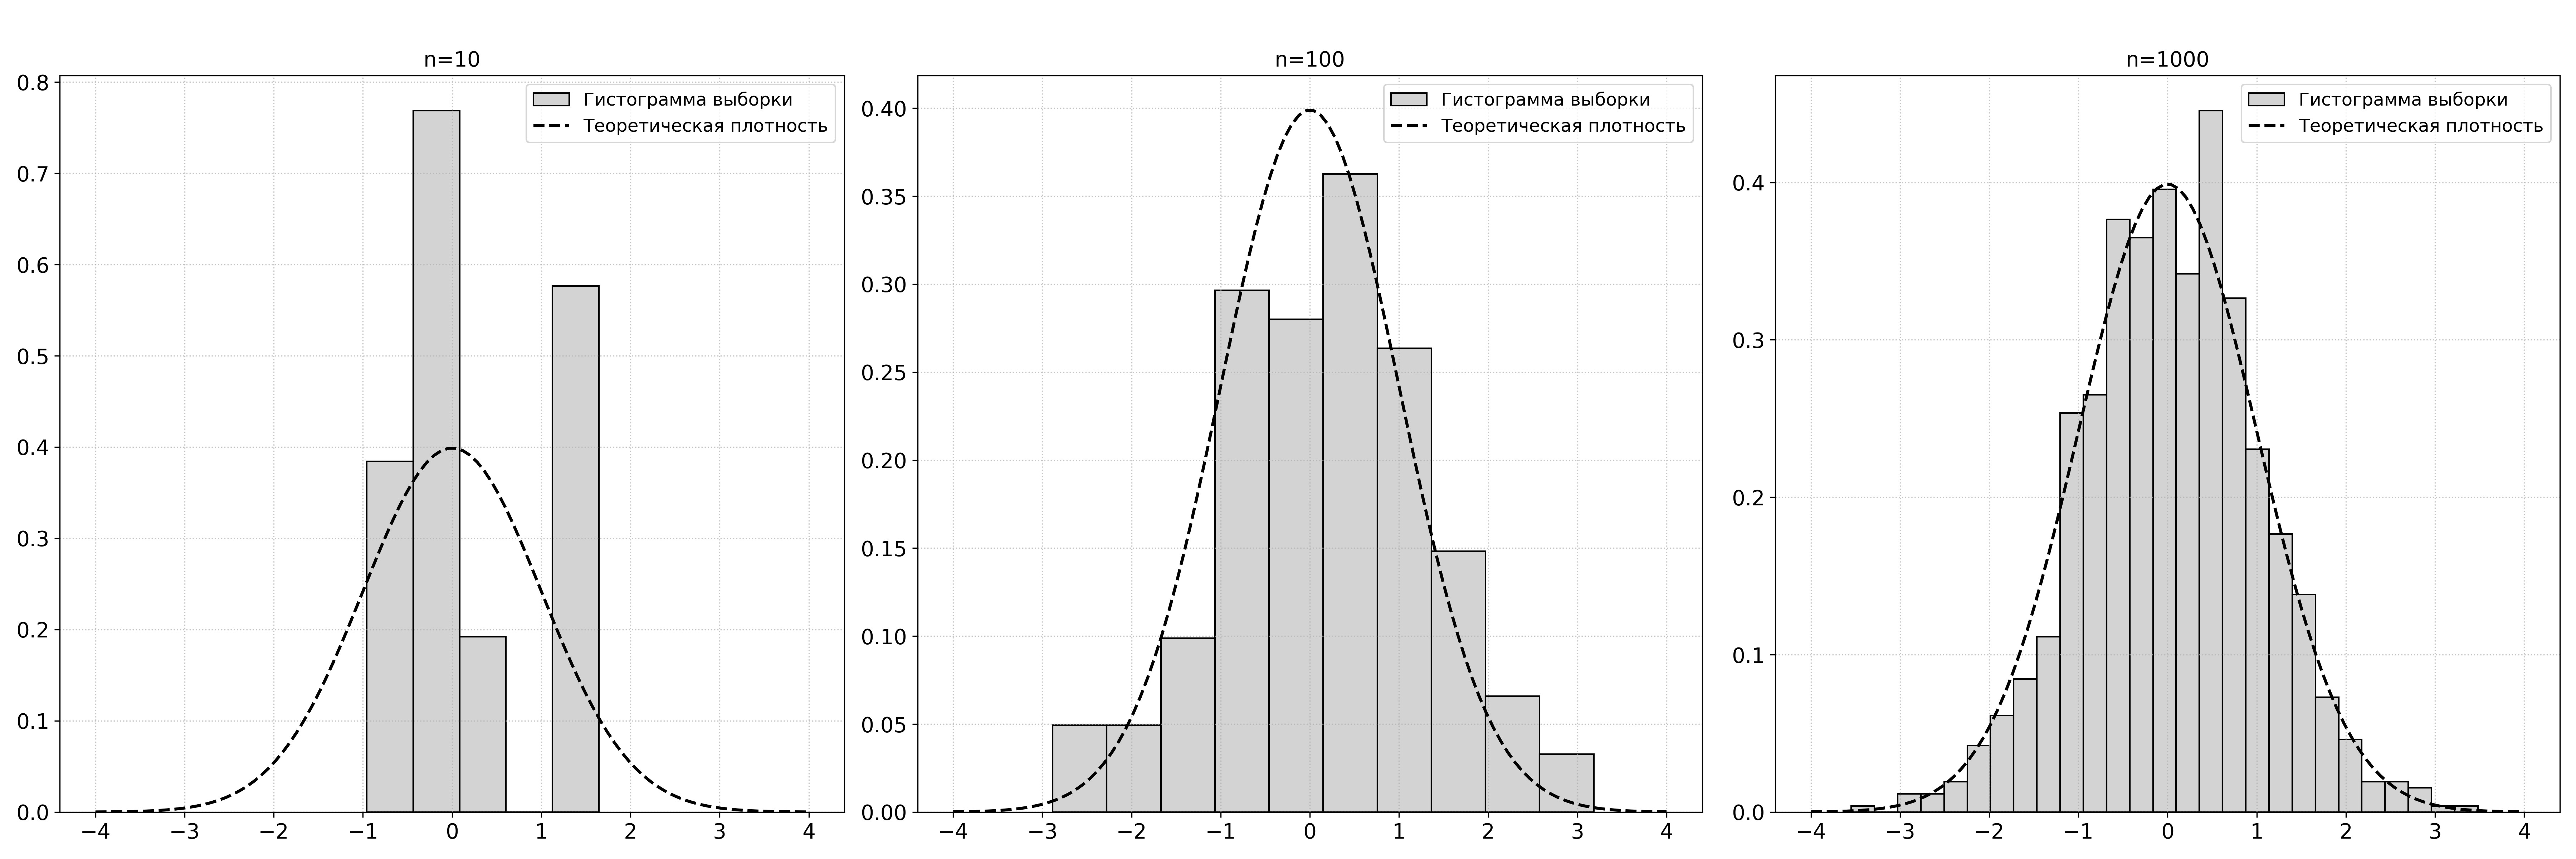
\includegraphics[width=\textwidth]{../figures/norm.png}
    \caption{Гистограмма и теоретическая плотность нормального распределения $N(0, 1)$}
    \label{fig:norm}
\end{figure}

\begin{figure}[H]
    \centering
    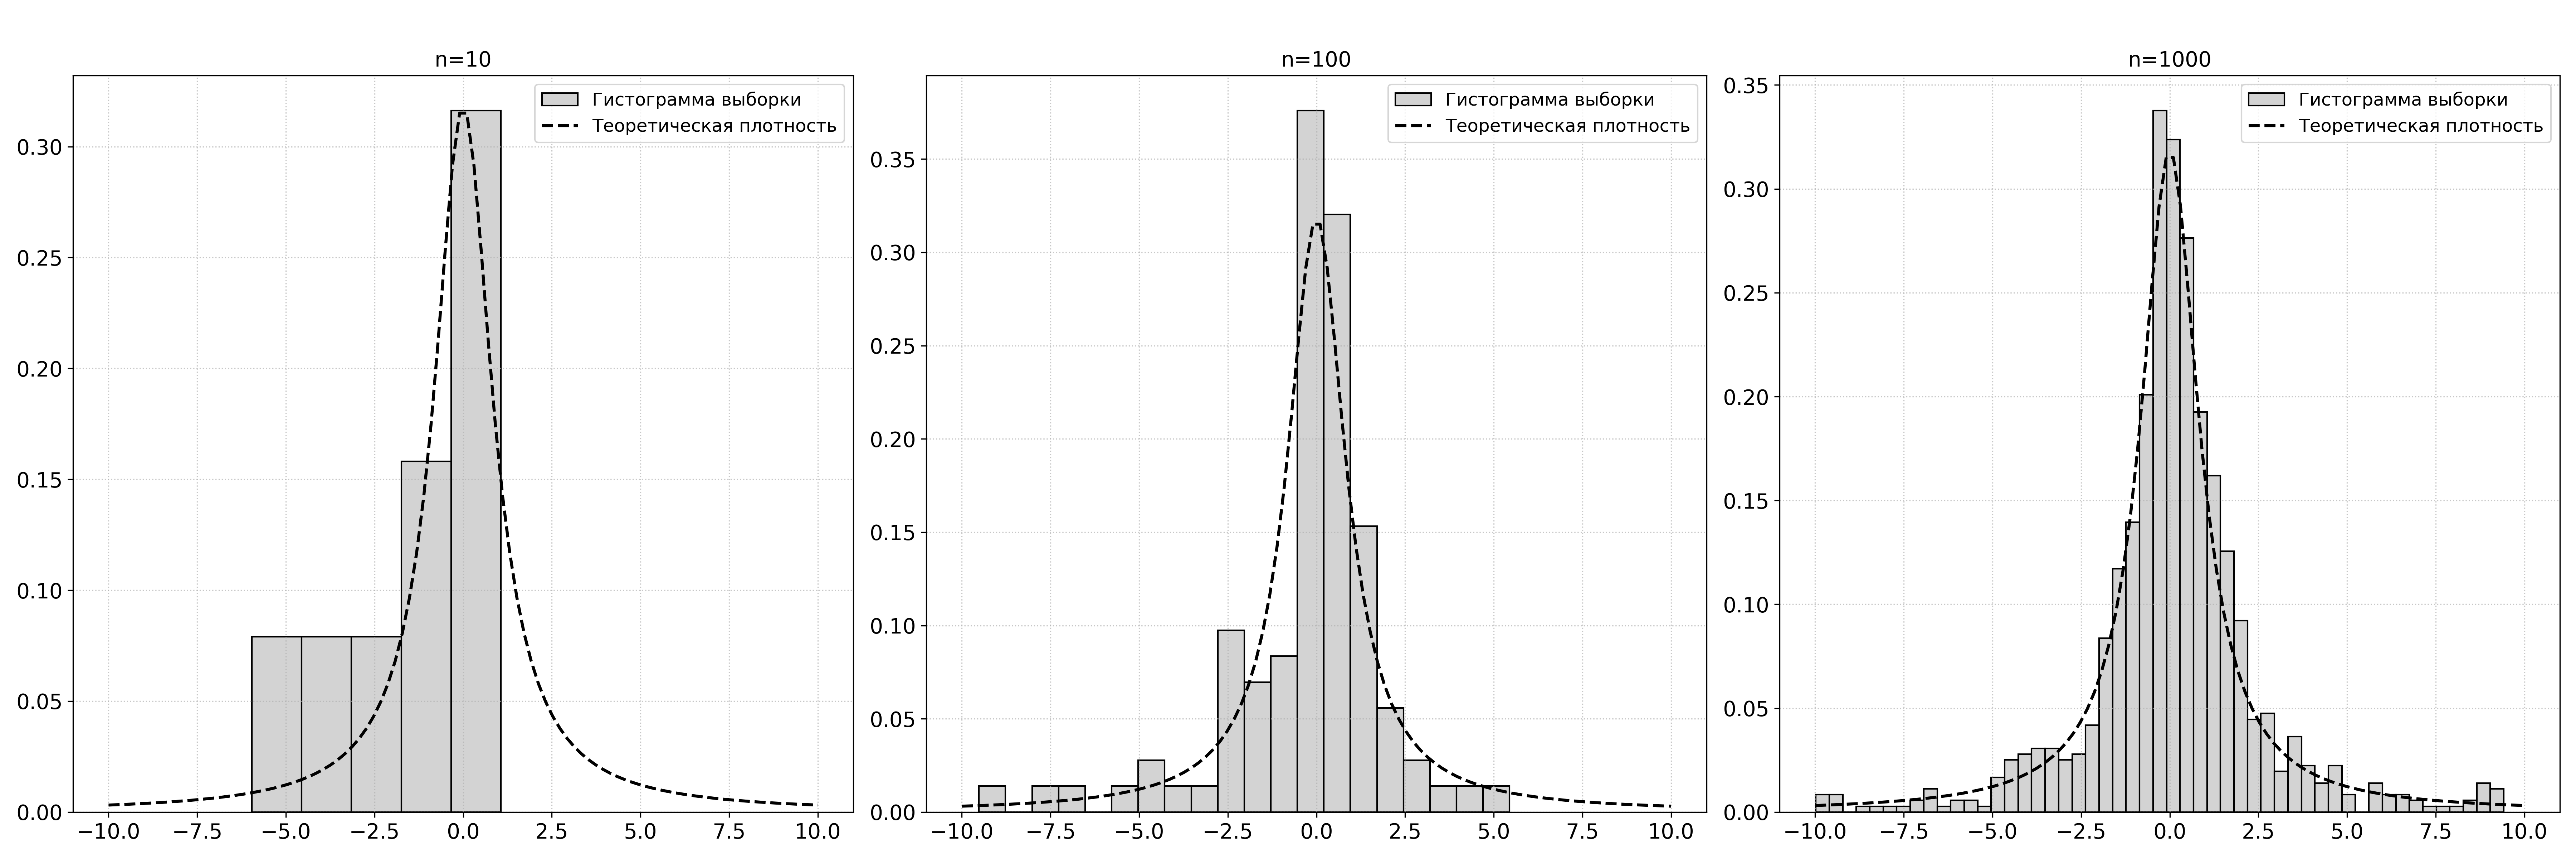
\includegraphics[width=\textwidth]{../figures/cauchy.png}
    \caption{Гистограмма и теоретическая плотность распределения Коши $C(0, 1)$}
    \label{fig:cauchy}
\end{figure}

\begin{figure}[H]
    \centering
    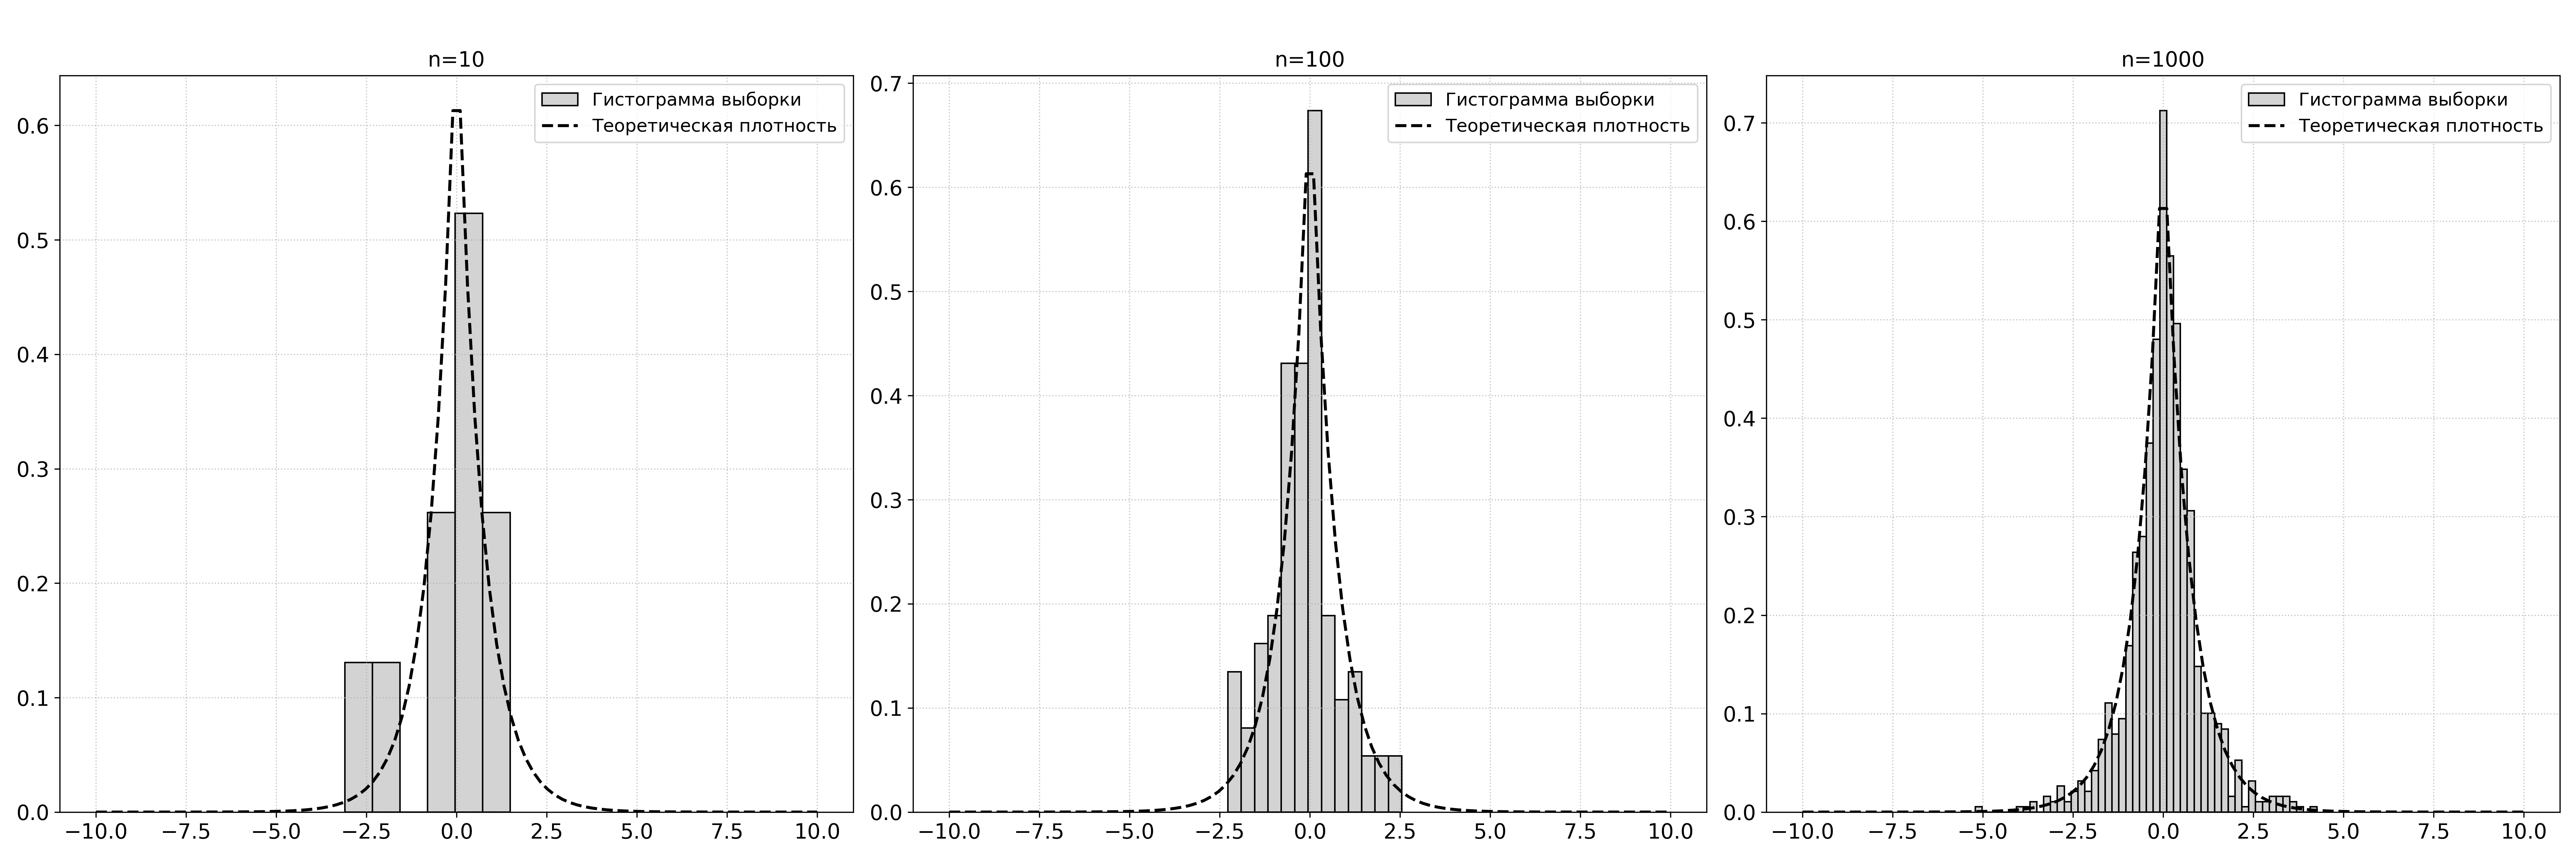
\includegraphics[width=\textwidth]{../figures/laplace.png}
    \caption{Гистограмма и теоретическая плотность распределения Лапласа $L(0, 1/\sqrt{2})$}
    \label{fig:laplace}
\end{figure}

\begin{figure}[H]
    \centering
    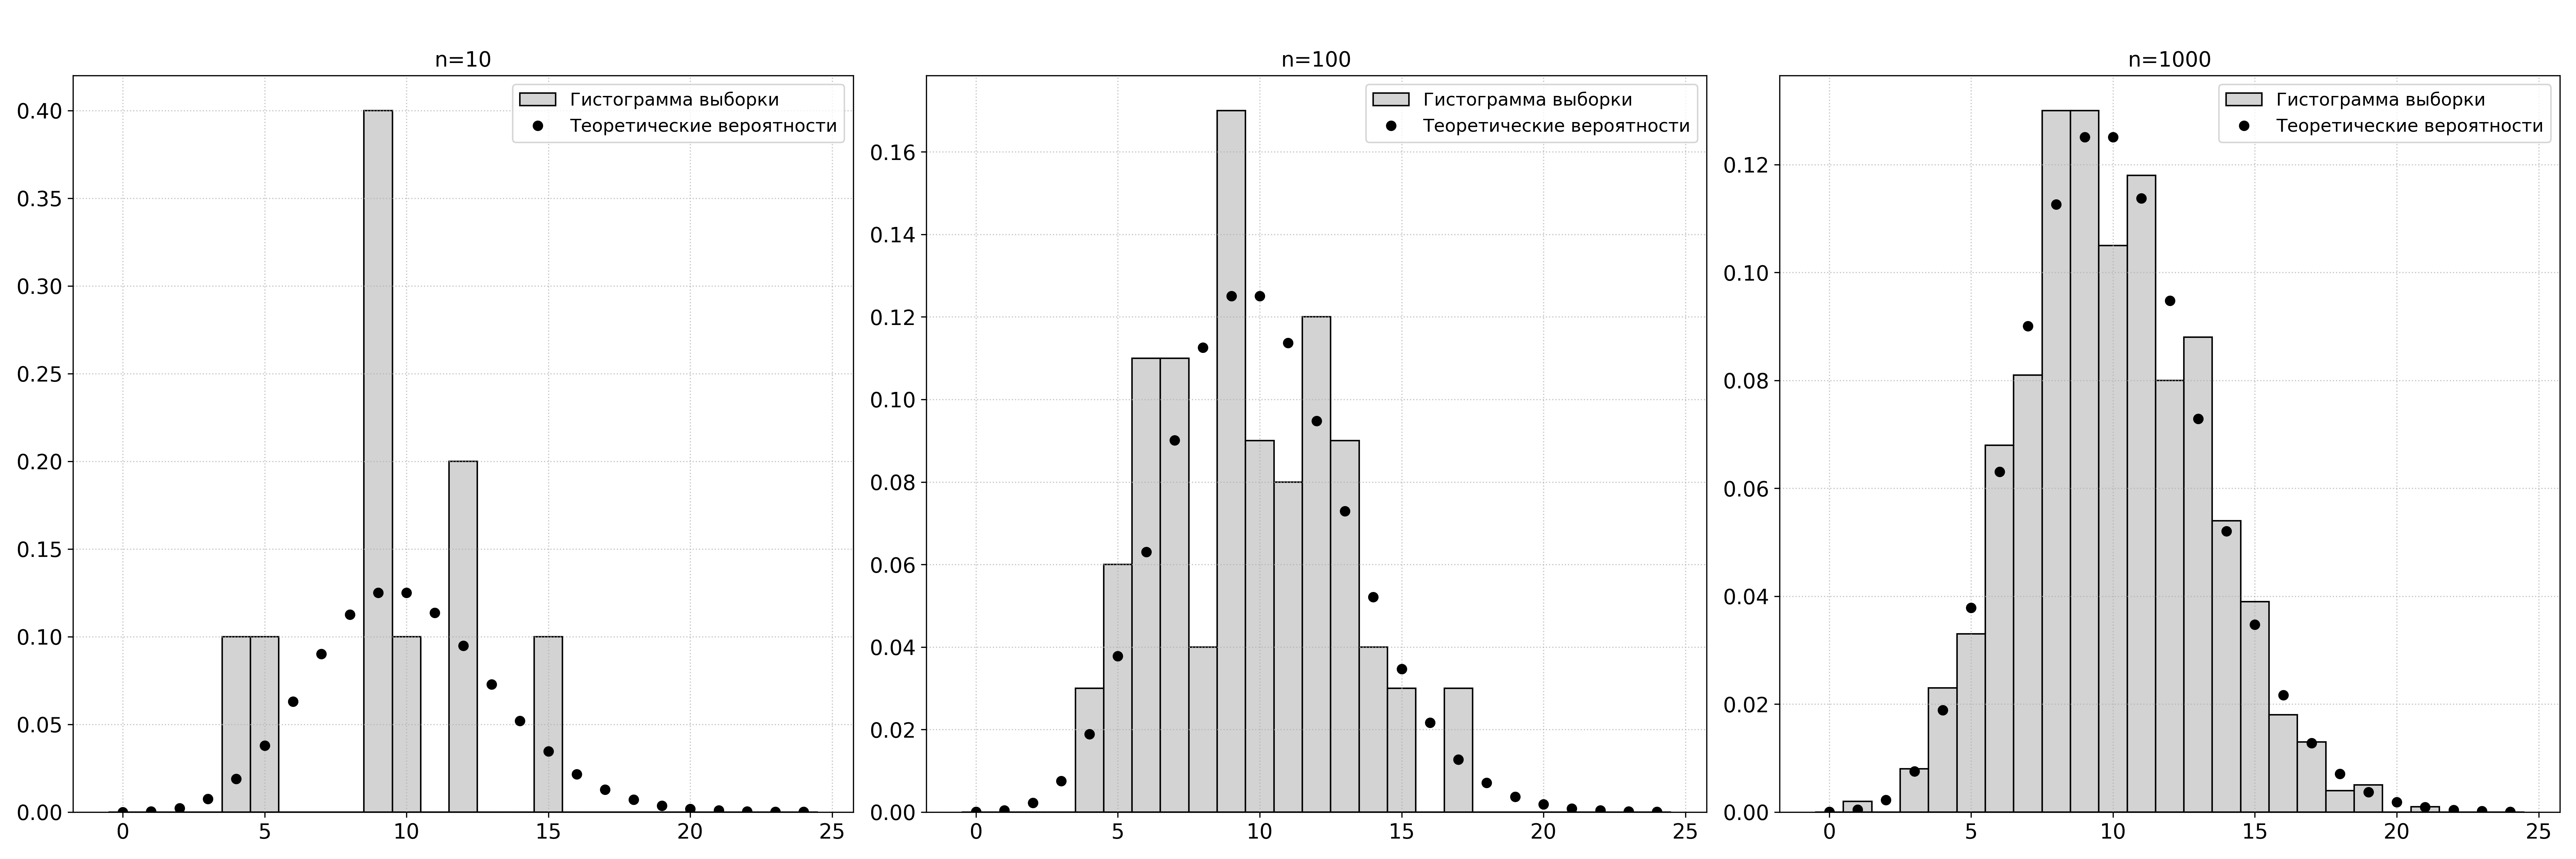
\includegraphics[width=\textwidth]{../figures/poisson.png}
    \caption{Гистограмма и теоретические вероятности распределения Пуассона $P(10)$}
    \label{fig:poisson}
\end{figure}

\begin{figure}[H]
    \centering
    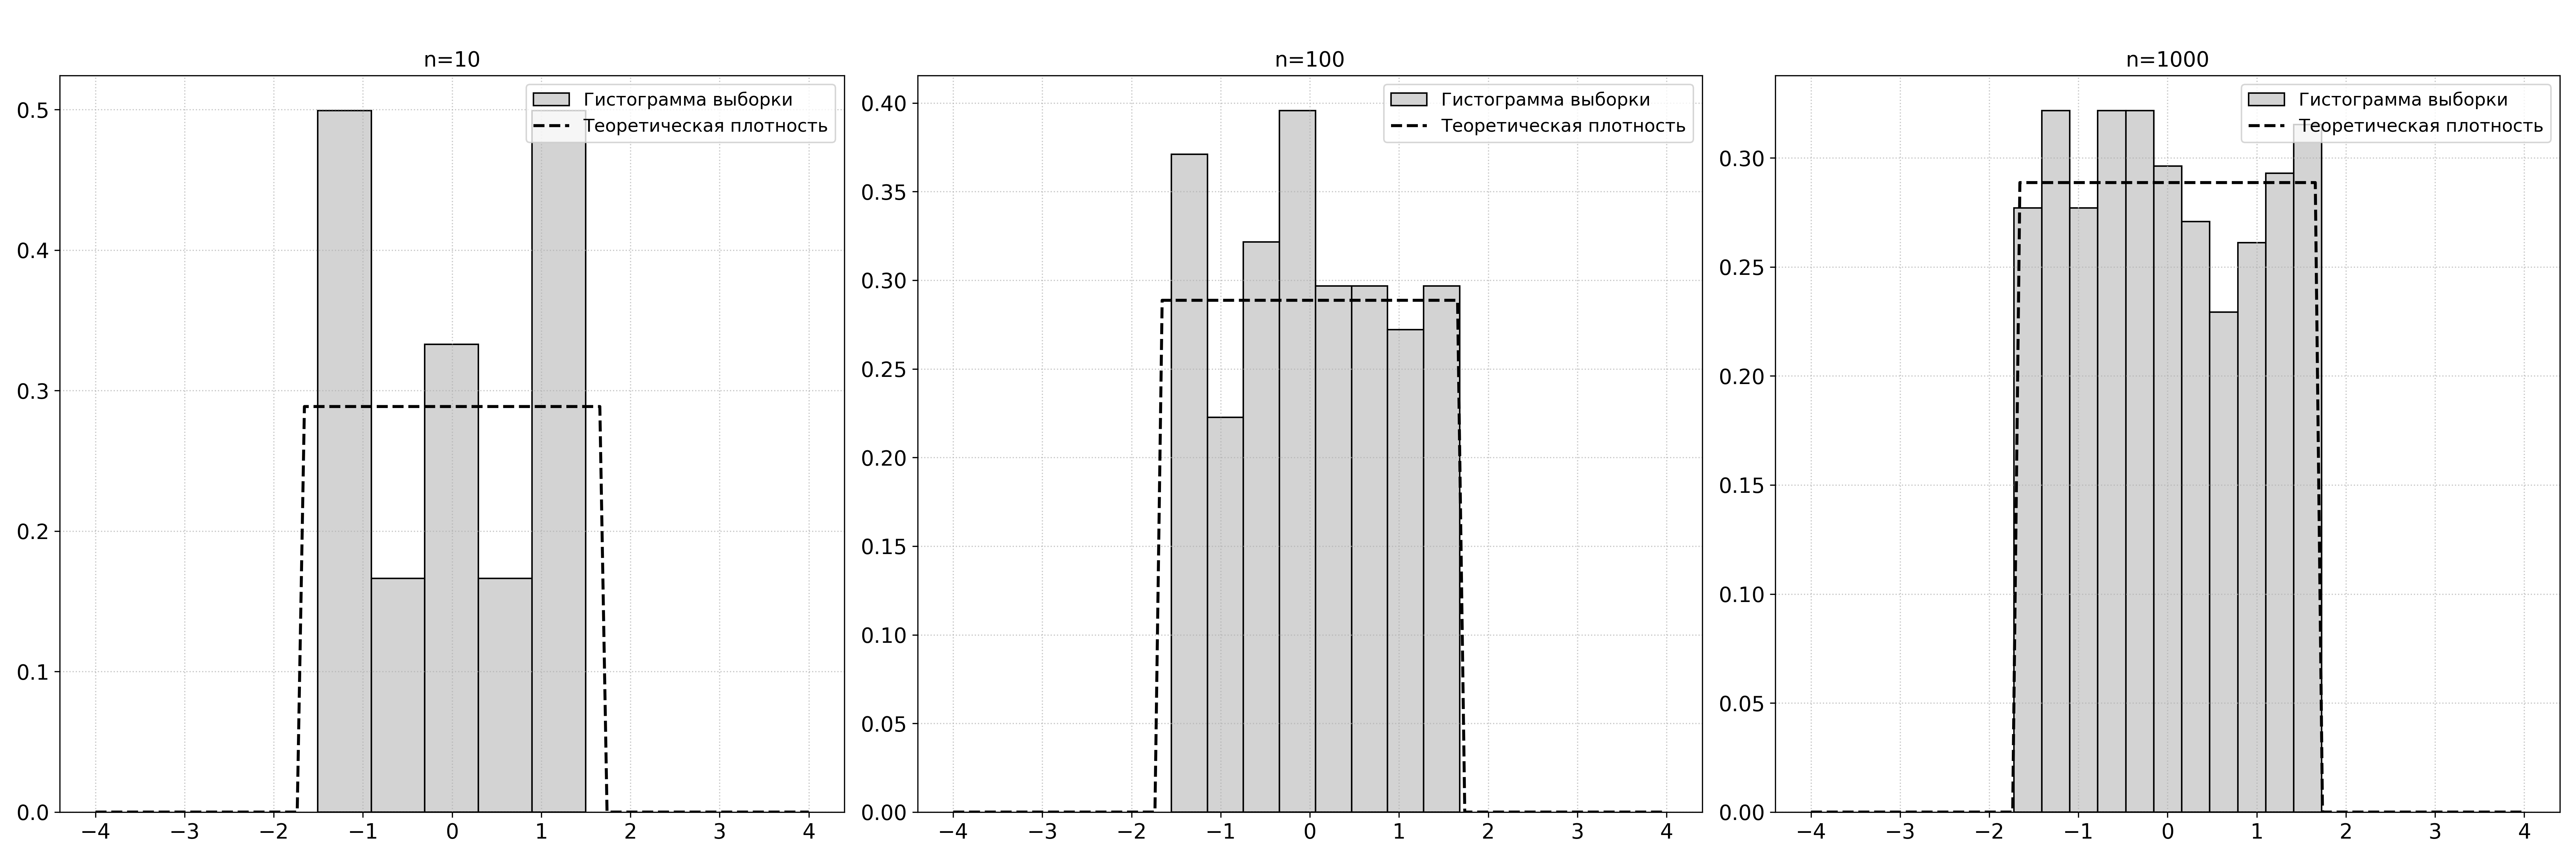
\includegraphics[width=\textwidth]{../figures/uniform.png}
    \caption{Гистограмма и теоретическая плотность равномерного распределения $U(-\sqrt{3}, \sqrt{3})$}
    \label{fig:uniform}
\end{figure}

\section{Обсуждение}

Анализ полученных графиков (рис.~\ref{fig:norm}--\ref{fig:uniform}) показывает, что с ростом объема выборки эмпирические гистограммы закономерно приближаются к теоретическим кривым. Такая картина наблюдается для всех рассмотренных распределений, хотя выражена по-разному в зависимости от их свойств.

При $n=10$ форма гистограмм в большинстве случаев определяется случайными колебаниями частот. Для нормального, лапласовского и равномерного распределений общий вид закона угадывается слабо. Для распределения Пуассона при таком объеме выборки отдельные столбцы заметно «скачут», поэтому судить о положении центра и форме распределения по одной реализации затруднительно.

При $n=100$ структура распределений становится более читаемой: у нормального распределения появляется характерная симметричная форма, у распределения Лапласа заметен более выраженный центральный пик, у равномерного распределения гистограмма становится ближе к постоянному уровню на заданном интервале. Для распределения Коши основная масса значений концентрируется около нуля, но влияние тяжелых хвостов по-прежнему заметно. В программной реализации для этого случая использовалось ограничение диапазона визуализации $[-10,10]$, что позволило корректно сравнить центральную часть эмпирических данных с теоретической плотностью.

При $n=1000$ наблюдается наилучшее согласование с теорией. Особенно наглядно это видно для нормального и равномерного распределений. Для распределения Пуассона при большом объеме выборки дискретная структура сохраняется, но относительные частоты уже близки к теоретическим вероятностям.

Таким образом, практический эксперимент подтверждает теоретическое положение: чем больше объем выборки, тем надежнее гистограмма отражает истинный закон распределения и тем обоснованнее последующие статистические выводы \cite{babakhina, maksimov}.

\section{Выводы}

В работе были реализованы генерация выборок и построение гистограмм для пяти распределений: нормального, Коши, Лапласа, Пуассона и равномерного. Сравнение с теоретическими кривыми показало, что при малом объеме выборки ($n=10$) форма гистограммы сильно зависит от случайных колебаний и не всегда позволяет уверенно определить тип распределения.

При увеличении объема выборки до $n=100$ и особенно до $n=1000$ гистограммы становятся более устойчивыми, а их форма заметно лучше согласуется с теоретическими плотностями (и вероятностями для распределения Пуассона). Следовательно, для надежной визуальной интерпретации распределения необходим достаточно большой объем данных.
 
\refstepcounter{section}
\addcontentsline{toc}{section}{\thesection\ Список литературы}
\renewcommand{\refname}{\thesection\ Список литературы}

\begin{thebibliography}{9}

    \bibitem{babakhina}
    Бабахина С. А., Баженов А. Н. Практикум по математической статистике: учеб. пособие. — СПб. : Санкт-Петербургский политехнический университет Петра Великого, 2026. 

    \bibitem{maksimov}
    Максимов Ю. Д. Математика. Теория и практика по математической статистике. Конспект-справочник по теории вероятностей : учеб. пособие. — СПб. : Изд-во Политехн. ун-та, 2009. — 395 с. 

\end{thebibliography}

\section{Приложение}

Исходный код программ доступен в репозитории на GitHub: \\
\url{https://github.com/Reichenau/math-stats-labs}
 
\end{document}
